\chapter{Background}
This chapter presents the background of the thesis. On the one hand we describe the RoboCup and LLSF in section 2.1 and the Robotino in section 2.2. On the other hand we present the most important software for this thesis. These are the two robot software frameworks ROS and Fawkes in section 2.3. Section 2.4 describes the data exchange format Protocol Buffers, following with the robot simulator Gazebo in section 2.5 and the document database MongoDB in section 2.6.


\section{RoboCup}
The \textit{RoboCup}\footnote{\url{http://www.robocup.org}} is an international robotics competition founded in 1997~\cite{Robocup}. It provides standard problems as a platform for artificial intelligence and robotics research. Research teams from all over the world compete in different leagues to benchmark their robotic system. The RoboCup fosters important research results because the participating teams realize theoretic approches and make them robust against the challenges of the real world complexity. Furthermore the competition leads to comperison and evaluation of different approches. Every jear there the competition takes place at the RoboCup world championship, which is hosted by changing nations. There are also offshoots, such as the RoboCup GermanOpen in Magdeburg.\\
Initially, the RoboCup started as robot soccer world cup. The goal ``By mid-21st century, a team of fully autonomous humanoid robot soccer players shall win the soccer game, comply with the official rule of the FIFA, against the winner of the most recent World Cup.''~\cite{robocup_goal} shows how far the RoboCup is going to push the development of artificial intelligence and robotics. The RoboCup has grown and features now a variaty of different leagues in different domains. The following gives an overview over the RoboCup leagues in 2013:\\
\textbf{Soccer Leagues:} The majority of the RoboCup leagues are soccer leagues with different sizes and platforms. There is a standart platform league where the teams have to use the about 60 cm high Nao robot without any hardware modifications. This enables the teams to concentrate on vision, behavior and motion tasks. There is also a league for humanoid robots. This league is devided in three subleagues with kid, teen and adult size robots. The middle size league features up to five robots with a footprint smaller than 52cm x 52cm per team and a 18 m x 12 m field. In the small size league, there are six robots with a diameter up to 18 cm per team. There are also two simulation leagues which focus artificial intelligence and team strategy instead of developing robot hardware. There are a 2D simulation league and a 3D simulation league. In the 3D simulation league teams consisting of eleven virtual Nao robots compete against each other in a realistic soccer environment. \textcolor{red}{In the related work}, we will show this simulation in detail.\\
\textbf{RoboCup @Home:} The RoboCup @Home league is a competition about service robots. The robots have to assist humans in a domestic environment. There are a variaty of tasks such as following a human, serving drinks and handling emergency situations. Especially imprtant in this league are the techical and open challenge. Here the teams can present their own ideas and how the robot solves it.\\
\textbf{Rescue League:} The rescue league is a testbed for urban search and rescue robots. The robots have to find victims in a parkour that simulates an urban area after an earthquake. This league also has a simulation offshoot we show in the chapter about the \textcolor{red}{related work}.\\
\textbf{Robocup @Work:} The RoboCup @Work league targets working tasks with the YouBot. The YouBot is a mobile robot with an advanced manipulator. The goal is to perform work-related tasks such as identifying and handleing different objects, placing them in bins and transportation.\\
\textbf{Logistic League:} We describe this league in detail in the following subsection.\\

\subsection{Logistic League sponsored by Festo}
The Logistic League Sponsored by Festo (LLSF) is a competition in the RoboCup. LLSF aims to foster scientific work on autonomous solutions for logistics and to provide a testbed for existing approaches~\cite{LLSFTestbed}. The participants should find new approaches and improve already existing ones to optimize material and information flow in logistics.
LLSF takes place  in a simplified production hall~\cite{LLSFRules}.
\begin{figure}
\begin{minipage}[b]{0.5\linewidth}
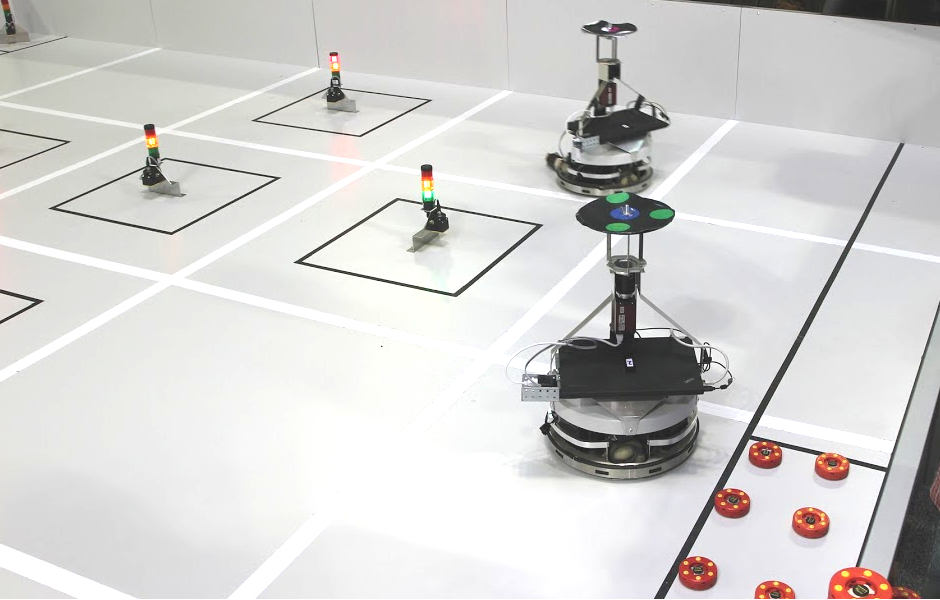
\includegraphics[scale=0.23]{pics/llsf}
\caption{Part of the LLSF field}
\label{fig:llsf_field}
\end{minipage}
\quad
\begin{minipage}[b]{0.5\linewidth}
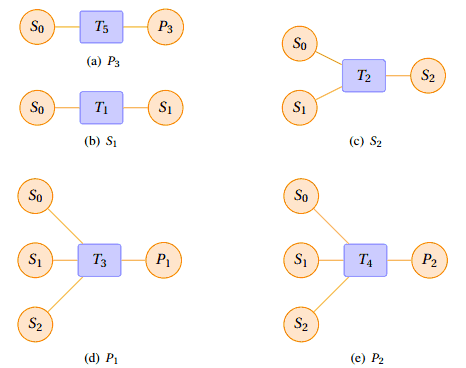
\includegraphics[scale=0.45]{pics/production_chain}
\caption{LLSF Production Chain}
\label{fig:llsf_chain}
\end{minipage}
\end{figure}
Figure~\ref{fig:llsf_field} shows a part of the 5.6m x 5.6m hall with
two Carologistic robots, three machines and some material-pucks. The
main task of LLSF is to produce and deliver ordered products as
efficient as possible by feeding machines with resources and
semi-finished products. The participants can use up to three Robotino
robots by Festo~\cite{{Robotino}}. We present the Robotino in the next
section in detail. Orange pucks represent resources and products. They
are equipped with an RFID-chip\footnote{Radio-frequency identification
  allows the wireless identification of objects with small chips.}
which is needed to store the different product states of the
pucks. The machines are represented by the RFID-readers with the
traffic light on top. The traffic-light indicates the current status
of a machine, such as ready, producing and out-of-order. The machines
take ressources and semi-finished products as input and turn one input
uck in a further produced puck. All other inputted pucks are turned
into consumed puck which can be recycled to get new ressource
pucks. There are different types of machines. The type defines the
needed input and the produced output of a
machine. Figure~\ref{fig:llsf_chain} shows the production chain. There
are the raw-material pucks $S0$, intermidiate product pucks $S1$ and $S2$
and product puck $P1$, $P2$ and $P3$. The machine types are labled with
$T1$ to $T5$. Beside these regular machines there are also Recycling
machines which turn consumed pucks into raw-material pucks and
delivery machines which only take finished product pucks. The team gets awarded with points for delivering finished products, producing complex pucks and recyling. The game is devided in two phases. In the first phase, the \textit{exploration phase}, the robots have three minutes to explore the production area to identify which machine has which type. The team also receives points for each correct reported machinetype. The second phase is the actual \textit{production phase} and lasts 15 minutes. The league also features an automated referee box (refbox). It controls the machines and communicates with the robots during the game. The refbox gives orders which products are to be produced, informs the robots about the game state and rewards points for achieved goals.


\section{Robotino}
The \textit{Robotino}~\cite{Robotino} is a mobile robot developed by Festo Didactic~\footnote{http://www.festo-didactic.com}. It is used for research and education. The shape of the robotino is a cylinder with 37cm diameter and 21cm height. It holds omni-directional wheels to be able to drive in any direction and turn at the same time. It is shipped with nine infrared distance mesuring sensors ordered around the robot, a bumper around the robot to detect collisions and a webcam. A microcontroller and an embedded PC with 800 MHz and 128 MB RAM are used to control the robot. The PC runs with a linux Operating System. The Robotino is designed to be extendable to be usable in different applications. Therefore additional sensors and actuators can be attached. In the front of the Robotino, there is a loading bay with some space for extensions. Some common extensions are a forklift, a static gripper to move pucks on the ground and a laser range finder.\\
\textcolor{red}{In LLSF, we use the Robotino shown in figure dingdong.}


\section{Robot Software Frameworks}
\subsection{Robot Operating System}
The \textit{Robot Operating System (ROS)}~\cite{Ros} is an Open Source framework designed to operate on many robot platforms and to provide a standardized integration framework. It provides a collection of other useful Open Source libraries and tools for the development process of robot-software. Currently, it is widely used and has a large community. Each components integrated in ROS runs an own process and is called \textit{node}. ROS features peer-to-peer communication between the nodes. The nodes can register a publisher or subscriber to a specified \textit{topic}. If a publisher of a topic sends a message, every subscriber of same topic receives the message. We will describe the message protocol Google Protobuf used by ROS later. The communication is managed by a process called \textit{Roscore}. Roscore acts as a server. All nodes have to connect to the server in order to start.\\
We use ROS in LLSF for two reasons. First, we use ROS for motion planing. The ROS package \textit{Move Base} provides a global path planning and local motion planning with collision avoidance. We provide a global navigation graph for the LLSF field, the position and orientation of the robot, laser data for obstacle detection and motion goals by publishing messages to specified topics. With this data, Move Base computes a motor command. We subscribe to the motor command topic and send execute the command. Second, we use the \textit{Rviz} package for visualization. On the one hand we visualize incoming laser data and the localization of the robot in the LLSF field with all position hypotheses of our adaptive monte carlo localization (amcl). \textcolor{red}{erklären?}. On the other hand we visualize the global and local motion plan. Moreover, we use Rviz to send localization hints to amcl.

\subsection{Fawkes}
\textit{Fawkes} is an Open Source robot software framework developed primarily at the Knowledge-based Systems Group\footnote{\url{http://www.kbsg.rwth-aachen.de/}} (KBSG) at RWTH Aachen University. It is designed to run on multiple platforms and domains. It is written for Unix systems and follows a component-based software design~\cite{FawkesDesign}. It provides an infrastructure to load and unload binary components (implemented as \textit{plugins}) at run-time. Fawkes features a \textit{blackboard} as communication structure between the plugins. The blackboard lists structured entries called \textit{interfaces}. Pugins can read and write interfaces with a specified id. There can be many readers but only one writer for an interface. Furthermore Fawkes organizes plugin activity in threads to make use of multi-core architectures. Because of this design, Fawkes is flexible and dynamic. The interchangeability of the plugins, which is caused by the well defined interfaces, makes hardware abstraction and reuse easy. This is also an important advantage for the development of the simulation because the simulation can easily exchange the lower-level robot control and sense plugins. The robot control plugins on higher levels can operate as usual because the interface is the same. The features of Fawkes are provided with \textit{aspects}. These aspects are based on aspect-oriented programming~\cite{aspect_oriented} and give access to a particulat feature. Threads that want to use a feature can inherit from the corresponding aspect. For example there are aspects for accessing the blackboard, logging and timing~\cite{tnthesis}. In this thesis, we provide communication with the simulation by using such an aspect. Two other important features for this thesis are the centralized clock and the configuration. The centralized clock provides the time for all plugins. Especially important for this thesis is the possibility to give Fawkes an alternative timesource. So, it is easy to exchange the the system time with the simulation time for all plugins without having to modify them. Also important for this thesis is the way Fawkes provides configurations. The configuration-files for all plugins are formated in the same format. A superordinate configutation file chooses which configuration files have to be loaded. There is the possibility to start Fawkes with a specified configuration by seting a superordinate configuration file. Furthermore there is the possibility to override configuration values.\\
In comparison to ROS, the advantage of Fawkes is the tighter integration of the used components. The main loop of Fawkes controls the execution order of all component threads. This makes it possible to match certain time criteria for the components and to provide a \textit{sense-think-act} cycle.\\
We use Fawkes as our main robot software framework. Nearly all software components for our robot are integrated as plugins in Fawkes. Therefore, in this thesis, we have to provide the sensor data from the simulation and get commands for the actuators in Fawkes.

\textcolor{red}{Clock}

\textcolor{red}{Configurations}

\textcolor{red}{Plugins used???}

\section{Gazebo}
\section{Additional Software}
\subsection{Protocol Buffers}
\subsection{MongoDB}
